\subsection{Запуск проектов}
\subsubsection{Технические характеристики}
Исполнение существующих проектов осуществлялось с помощью файла \texttt{inference.py}, который доступен в каждом из рассматриваемых проектов. В контексте машинного обучения, \texttt{inference} означает оценку результативности модели на похожих данных. В этом состоянии модель не обучается и не тестируется, а лишь выдаёт результаты, под которые ранее происходило обучение.

В силу нехватки вычислительных ресурсов, а также высоких системных требований у диффузионных моделей, по мере проведения экспериментов всё более актуальных \texttt{SOTA} (state of the art) моделей, требуется больше вычислительных ресурсов. Данное замечание является серьёзным недостатком решений \texttt{LaDI"=VITON} и \texttt{PromptDresser}. Таблицу с характеристиками вычислительных машин для каждого из рассматриваемых решений можно увидеть в таблице \ref{tab:tech_models}.


\begin{table}[H]
\small
\begin{tabularx}{\linewidth}{lXXX}
      & PASTA-GAN++ & LaDI-VITON & PromptDresser \\
\hline
GPU  & GeForce GTX 1060 3GB & GeForce RTX 2060 8GB & GeForce GTX 1070 8GB \\
CPU  & Intel Core i5-6400   & AMD Ryzen 7 2700 AM4     & Intel Core i5-8400 \\
RAM  & 16GB DDR4     & 16GB DDR4       & 32GB DDR4 \\
\end{tabularx}
\caption{Технические характеристики вычислительных машин для каждой из моделей. Несмотря на разницу в вычислительных ресурсах, \texttt{PromptDresser} требует значительно больше времени для генерации изображений.}
\label{tab:tech_models}
\end{table}


В рамках оценивания результатов использовались такие метрики, как \texttt{LPIPS} и \texttt{FID}. Они являются наиболее предпочтительными на фоне \texttt{MSE} и подобных функций, поскольку позволяют сравнивать изображения на основе не просто пикселей, а более глубоких признаков, таких как яркость и цветной состав.

\subsubsection{FID}
\texttt{FID} (Fréchet Inception Distance) представляет собой метрику, которая оценивает сходство между двумя наборами изображений путем сравнения их статистических характеристик в пространстве признаков. Таким образом, \texttt{FID} сравнивает распределение сгенерированных изображений с распределением изображений из исходного набора данных. Данная метрика вычисляется с помощью формулы, которая представляет собой 2"=Wasserstein расстояние между двумя многомерными гауссовскими распределениями \cite{fid}:
\begin{gather}
FID(\mu_r, \Sigma_r, \mu_g, \Sigma_g) = ||\mu_r - \mu_g||_2^2 + Tr(\Sigma_r + \Sigma_g - 2(\Sigma_r \Sigma_g)^{\frac{1}{2}}),
\end{gather}
где $(\mu_r, \Sigma_r)$ есть выборочное среднее и ковариационная матрица реальных признаков, $(\mu_g, \Sigma_g)$ "--- выборочное среднее и ковариационная матрица сгенерированных признаков, $Tr(\cdot)$ представляет собой операцию взятия следа от матрицы.

Ключевым предположением \texttt{FID} является то, что распределения признаков как реальных, так и сгенерированных изображений могут быть аппроксимированы многомерными нормальными распределениями . Первое слагаемое в формуле $||\mu_r - \mu_g||_2^2$ измеряет квадрат евклидова расстояния между средними двух распределений . Второе слагаемое $Tr(\Sigma_r + \Sigma_g - 2(\Sigma_r \Sigma_g)^{1/2})$ учитывает различия в ковариационных структурах, что позволяет оценить разнообразие изображений в рассматриваемых наборах.

В рамках анализа, для вычисления \texttt{FID} были использованы библиотеки \texttt{torchvision}, \texttt{scipy} и \texttt{numpy} для исполнения операций из линейной алгебры, \texttt{PIL} для считывания изображений, \texttt{matplotlib} для визуализации результатов. Код программы, вычисляющей \texttt{FID}, можно увидеть в приложении \ref{app:fid}. Результаты вычисления метрики можно увидеть на рисунке \ref{fig:fid_results}. \cite{fid}.

\begin{figure}[H]
    \centering
    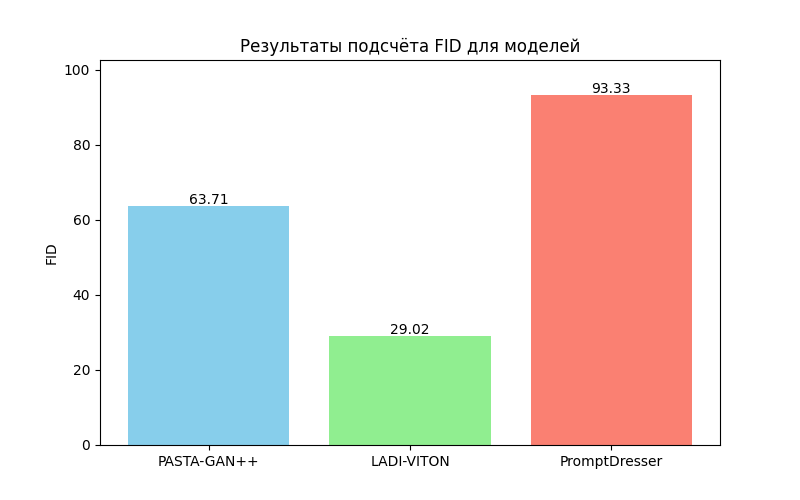
\includegraphics[width=0.85\linewidth]{images/fid_results.png}
    \caption{Результаты вычисления \texttt{FID}.}
    \label{fig:fid_results} 
\end{figure}

\subsubsection{LPIPS}
\texttt{LPIPS} (\texttt{Learned Perceptual Image Patch Similarity}) является оценкой цветового состава, текстуры и стиля. В основе метрики лежит использование предобученных сверточных нейронных сетей (например, \texttt{AlexNet}), которые извлекают из изображений карты признаков (feature maps) на различных уровнях абстракции. Для двух сравниваемых изображений вычисляются активации определённых слоёв сети, после чего производится их нормализация по канальному измерению.

Затем для каждой пары соответствующих карт признаков вычисляется евклидово расстояние, взвешенное специальными обучаемыми коэффициентами для каждого слоя. Итоговое значение \texttt{LPIPS} представляет собой сумму этих расстояний, усреднённую по всем слоям и пространственным координатам. Формула для рассчёта расстояния:
\begin{gather}
    d_l(x, y) = \frac{1}{H_lW_l}\sum_{h, w}||w_l \odot (\hat{F}(x)_{hw} - \hat{F}(y)_{hw}||_2^2,
\end{gather}
где $w_l$ "--- веса для слоя $l$.

Таким образом, формула \texttt{LPIPS} выглядит следующим образом:
\begin{gather}
    LPIPS(x, y) = \sum_{l \in L}d_l(x, y)
\end{gather}

Методы нормализации, представленные в виде $\hat{F}(\cdot)$, гарантируют минимизацию влияния масштаба каждого канала из карты признаков. Низкие значения \texttt{LPIPS} соответствуют высокой степени визуального сходства, а большие значения указывают на значительные различия между изображениями. Это делает \texttt{LPIPS} предпочтительной метрикой для оценки качества изображений, полученных с помощью генеративных моделей, поскольку она лучше отражает субъективное качество, чем классические метрики.

\begin{figure}[H]
    \centering
    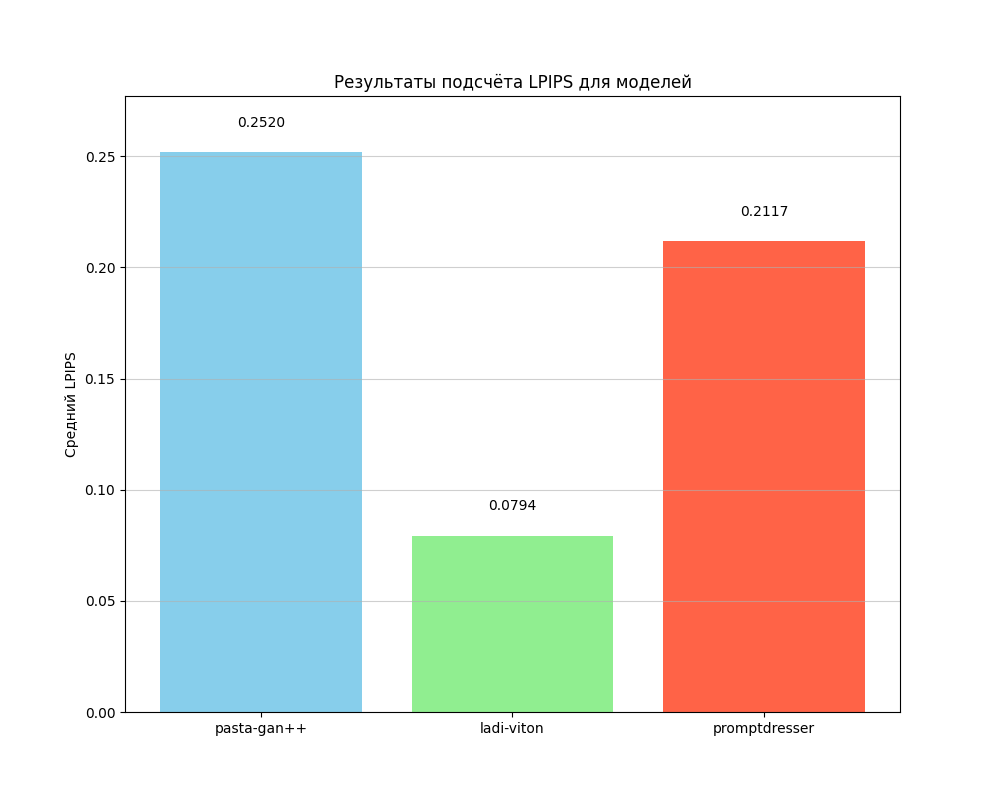
\includegraphics[width=0.9\linewidth]{images/lpips_results.png}
    \caption{Результаты вычисления \texttt{LPIPS}.}
    \label{fig:lpips_results} 
\end{figure}

Реализация метрики осуществлялась с помощью \texttt{PyTorch}, \texttt{numpy} для работы с массивами данных, \texttt{matplotlib} для визуализации результатов, а также с помощью вспомогательной библиотеки \texttt{lpips}. Код вычисления метрики можно увидеть в приложении \ref{app:lpips}, результаты можно увидеть на изображени \ref{fig:lpips_results} \cite{lpips}.

\subsection{Анализ результатов}
Согласно полученным экспериментальным данным, диффузионная модель \texttt{LaDI"=VITON} продемонстрировала превосходящие результаты по сравнению с генеративно"=состязательной архитектурой \texttt{PASTA"=GAN++} и текстово"=управляемой системой \texttt{PromptDresser}. Успех данного подхода обусловлен фундаментальными преимуществами диффузионных моделей перед альтернативными архитектурами. Диффузионные модели осуществляют генерацию изображений посредством итеративного процесса удаления шума, что позволяет им более точно моделировать сложные распределения данных и генерировать фотореалистичные изображения. Несмотря на превосходящие результаты, диффузионные модели характеризуются значительно более высокими вычислительными требованиями по сравнению с альтернативными подходами.

Однако каждый из подходов имеет свои особенности, преимущества и ограничения в контексте их архитектурных решений.
\texttt{PASTA"=GAN++} продемонстрировала худшие результаты в сравнении с диффузионной моделью, однако и требование к вычислительной машине соответственно тоже значительно ниже. Данные результаты объясняются фундаментальными проблемами, присущими \texttt{GAN}"=архитектурам, таким как нестабильность в обучении при доминации одной сети над другой. \texttt{PromptDresser}, реализующий подход генерации одежды на основе текстовых запросов, столкнулся проблемой в сложности точного перевода текстовых описаний в визуальные характеристики одежды, особенно для сложных атрибутов, таких как текстура, стиль посадки и детали кроя.
